\hypertarget{index_overview}{}\section{Elektra Initiative Overview}\label{index_overview}
Elektra provides a universal and secure framework to store configuration parameters in a global, hierarchical key database. The core is a small library implemented in C. The plugin-\/based framework fulfills many configuration-\/related tasks to avoid any unnecessary code duplication across applications while it still allows the core to stay without any external dependency. Elektra abstracts from cross-\/platform-\/related issues with an consistent A\+P\+I, and allows applications to be aware of other applications' configurations, leveraging easy application integration.

See the website for more information \href{http://www.libelektra.org}{\tt http\+://www.\+libelektra.\+org}\hypertarget{index_focus}{}\section{A\+P\+I docu}\label{index_focus}
This document occupies with the A\+P\+I implementation, documentation, internals and plugins. On the one hand it gives an overview and an introduction for developers using Elektra, on the other hand it gives an informal descriptions what methods must and may provide to allow an alternative implementation of the A\+P\+I.

The current version (for stable releases) of this document can be found at \href{http://doc.libelektra.org/api/current/html}{\tt http\+://doc.\+libelektra.\+org/api/current/html}

The latest version (from git master) of this document can be found at \href{http://doc.libelektra.org/api/latest/html}{\tt http\+://doc.\+libelektra.\+org/api/latest/html}\hypertarget{index_using}{}\section{Using the Elektra Library}\label{index_using}
A C or C++ source file that wants to use Elektra should include\+: 
\begin{DoxyCode}
\textcolor{preprocessor}{#include <kdb.h>}
\end{DoxyCode}


To link an executable with the Elektra library, one way is to use the {\ttfamily pkg-\/config} tool\+: 
\begin{DoxyCode}
$ gcc -o application `pkg-config --cflags --libs elektra` application.c
\end{DoxyCode}


Another way is to use C\+Make\+: 
\begin{DoxyCode}
find\_package(Elektra REQUIRED)
include\_directories ($\{ELEKTRA\_INCLUDE\_DIR\})
target\_link\_libraries (application $\{ELEKTRA\_LIBRARIES\})
\end{DoxyCode}
\hypertarget{index_classes}{}\section{Elektra A\+P\+I}\label{index_classes}
The A\+P\+I was written in pure C because Elektra was designed to be useful even for the most basic system programs.

The A\+P\+I follows an object-\/oriented design, and there are 3 main classes as shown by the figure\+:


\begin{DoxyImage}
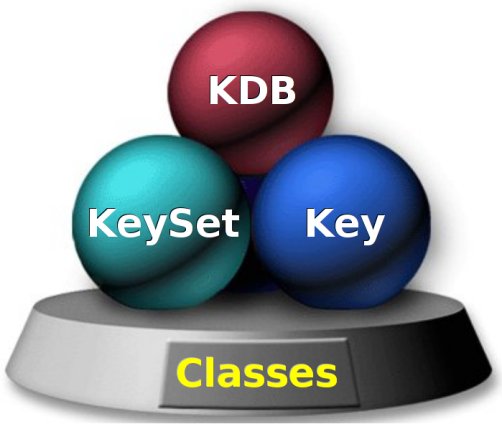
\includegraphics{classes.png}
\caption{Elektra Classes}
\end{DoxyImage}
 Some general things you can do with each class are\+:

\hyperlink{group__kdb}{K\+D\+B (Key Database) }
\begin{DoxyItemize}
\item \hyperlink{group__kdb_ga6808defe5870f328dd17910aacbdc6ca}{Open } and \hyperlink{group__kdb_gadb54dc9fda17ee07deb9444df745c96f}{Close } the Key Database
\item \hyperlink{group__kdb_ga28e385fd9cb7ccfe0b2f1ed2f62453a1}{Get } and \hyperlink{group__kdb_ga11436b058408f83d303ca5e996832bcf}{Set } \hyperlink{group__keyset}{Key\+Set } in the Key Database
\item See \hyperlink{group__kdb}{class documentation} for more
\end{DoxyItemize}

\hyperlink{group__key}{Key }
\begin{DoxyItemize}
\item \hyperlink{group__key_gad23c65b44bf48d773759e1f9a4d43b89}{Create } and \hyperlink{group__key_ga3df95bbc2494e3e6703ece5639be5bb1}{Delete }
\item Get and Set key the \hyperlink{group__keyname_ga7699091610e7f3f43d2949514a4b35d9}{name }
\item Get and Set \hyperlink{group__keyvalue_ga622bde1eb0e0c4994728331326340ef2}{string } or \hyperlink{group__keyvalue_gaa50a5358fd328d373a45f395fa1b99e7}{binary } values
\item Get and Set \hyperlink{group__keymeta}{Meta Data }
\item See \hyperlink{group__key}{class documentation} for more
\end{DoxyItemize}

\hyperlink{group__keyset}{Key\+Set }
\begin{DoxyItemize}
\item \hyperlink{group__keyset_ga671e1aaee3ae9dc13b4834a4ddbd2c3c}{Create } and \hyperlink{group__keyset_ga27e5c16473b02a422238c8d970db7ac8}{Delete }
\item Append \hyperlink{group__keyset_gaa5a1d467a4d71041edce68ea7748ce45}{a single key } or an entire \hyperlink{group__keyset_ga21eb9c3a14a604ee3a8bdc779232e7b7}{Key\+Set }
\item \hyperlink{group__keyset_ga317321c9065b5a4b3e33fe1c399bcec9}{Work with } its \hyperlink{group__keyset_ga4287b9416912c5f2ab9c195cb74fb094}{internal cursor }
\item See \hyperlink{group__keyset}{class documentation} for more
\end{DoxyItemize}\hypertarget{index_namespace}{}\section{Namespaces}\label{index_namespace}
There are 5 trees (=namespaces) of keys\+: {\ttfamily spec}, {\ttfamily proc}, {\ttfamily dir}, {\ttfamily user} and {\ttfamily system} that are all unified (in the given order) in one cascading tree starting with {\ttfamily /}.

The cascading tree is the logical tree to be used in applications. The other trees are the physical ones that stem from configuration sources. When using cascading key the best key will be searched at runtime, which appears like a tree on its own. See \hyperlink{group__keyset_cascading}{Cascading} in the documentation of \hyperlink{group__keyset_gad2e30fb6d4739d917c5abb2ac2f9c1a1}{ks\+Lookup\+By\+Name()} how the selection of keys works.


\begin{DoxyItemize}
\item The {\ttfamily spec} tree~\newline
 This tree specifies how the lookup should take place and also allows us to define defaults or document a key. The metadata of a key contains this information\+:
\begin{DoxyItemize}
\item {\ttfamily override/\#}\+: use these keys {\itshape in favour} of the key itself (note that {\ttfamily \#} is the syntax for arrays, e.\+g. {\ttfamily \#0} for the first element, {\ttfamily \#\+\_\+10} for the 11th and so on)
\item {\ttfamily namespace/\#}\+: instead of using all namespaces in the predefined order, one can specify which namespaces should be searched in which order
\item {\ttfamily fallback/\#}\+: when no key was found in any of the (specified) namespaces the {\ttfamily fallback}-\/keys will be searched
\item {\ttfamily default}\+: this value will be used if nothing else was found
\end{DoxyItemize}
\item The {\ttfamily proc} tree~\newline
 Is the only read-\/only tree. The configuration does not stem from the \hyperlink{group__kdb}{K\+D\+B (Key Database) }, but any other source, e.\+g. command-\/line arguments or environment.
\item The {\ttfamily dir} tree~\newline
 Allows us to have a per-\/directory overwrite of configuration files, e.\+g. for project specific settings.
\item The {\ttfamily user"} tree ~\newline
 Used to store user-\/specific configurations, like the personal settings of a user to certain programs. The user subtree will always be favoured if present (except for security concerns the user subtree may not be considered).
\item The {\ttfamily system} tree~\newline
 It is provided to store system-\/wide configuration keys, that is, the last fallback for applications but the only resort for daemons and system services.
\end{DoxyItemize}\hypertarget{index_rules}{}\section{Rules for Key Names}\label{index_rules}
When using Elektra to store your application's configuration and state, please keep in mind the following rules\+:
\begin{DoxyItemize}
\item You are not allowed to create keys right under the root. They are reserved for more generic purposes.
\item The keys for your application, called say {\itshape myapp}, should be created under {\ttfamily /sw/org/myapp/\#0/current} 
\begin{DoxyItemize}
\item sw is for software
\item org is the organisation. For uniqueness a full reverse url encoded with '/' instead of '.' is useful.
\item {\ttfamily \#0} is the major version of the configuration
\item current is the default configuration profile.
\item That means you just need to \hyperlink{group__kdb_ga28e385fd9cb7ccfe0b2f1ed2f62453a1}{kdb\+Get()} {\ttfamily /sw/org/myapp/\#0/profile} and then \hyperlink{group__keyset_gad2e30fb6d4739d917c5abb2ac2f9c1a1}{ks\+Lookup\+By\+Name()} in {\ttfamily /sw/org/myapp/\#0/profile/key} where profile is from command-\/line arguments and defaults to current.
\end{DoxyItemize}
\end{DoxyItemize}\hypertarget{index_backendsoverview}{}\section{Backend Overview}\label{index_backendsoverview}
The core of Elektra does not store configuration itself to the harddisk. Instead this work is delegated to backends.

If you want to develop a backend, you should already have some experience with Elektra from the user point of view. You should be familiar with the data structures\+: \hyperlink{group__key}{Key } and \hyperlink{group__keyset}{Key\+Set } Then you can start reading about Backends that are composed out of \hyperlink{group__plugin}{Plugins}. To get started with writing plugins, first read our plugin tutorial in doc/tutorials!\hypertarget{index_glossary}{}\section{Glossary}\label{index_glossary}

\begin{DoxyItemize}
\item {\bfseries pop}, used in \hyperlink{group__keyset_gae42530b04defb772059de0600159cf69}{ks\+Pop()} and \hyperlink{group__keyset_gga98a3d6a4016c9dad9cbd1a99a9c2a45aa52fb5f2cc86773d393da62bebebf7984}{K\+D\+B\+\_\+\+O\+\_\+\+P\+O\+P} means to remove a key from a keyset.
\item {\bfseries delete}, or abbr. del, used in \hyperlink{group__key_ga3df95bbc2494e3e6703ece5639be5bb1}{key\+Del()}, \hyperlink{group__keyset_ga27e5c16473b02a422238c8d970db7ac8}{ks\+Del()} and \hyperlink{group__keyset_gga98a3d6a4016c9dad9cbd1a99a9c2a45aa66a5380c120f25f28f49848c4a863ead}{K\+D\+B\+\_\+\+O\+\_\+\+D\+E\+L} means to free a key or keyset. The memory can be used for something else afterwards.
\item {\bfseries remove} means that the key/value information in the physical database will be removed permanently. 
\end{DoxyItemize}